\documentclass{beamer}
\usepackage[utf8]{inputenc}

\usetheme{Madrid}
\usecolortheme{default}
\useinnertheme{circles}

\definecolor{Logo1}{rgb}{0.208, 0.2865, 0.373}
\definecolor{Logo2}{rgb}{0.000, 0.674, 0.863}

\setbeamercolor*{palette primary}{bg=Logo1, fg=white}
\setbeamercolor*{palette secondary}{bg=Logo2, fg=white}
\setbeamercolor*{palette tertiary}{bg=white, fg=Logo1}
\setbeamercolor*{palette quaternary}{bg=Logo1,fg=white}
\setbeamercolor{structure}{fg=Logo1} % itemize, enumerate, etc
\setbeamercolor{section in toc}{fg=Logo1} % TOC sections

\usepackage{graphicx,animate}
%------------------------------------------------------------
%This block of code defines the information to appear in the
%Title page
\title[Linear Algebra] %optional
{Matrices and Gaussian Elimination}

\subtitle{Lecture 1}

\author[11910803@mail.sustech.edu.cn] % (optional)
{
    Zhang Ce
}

\institute[] % (optional)
{
    Department of Electrical and Electronic Engineering\\
    Southern University of Science and Technology
}

\date[2021.9.26] % (optional)
{2021.9.26}


%End of title page configuration block
%------------------------------------------------------------



%------------------------------------------------------------
%The next block of commands puts the table of contents at the
%beginning of each section and highlights the current section:

\AtBeginSection[]
{
\begin{frame}
    \frametitle{Table of Contents}
    \tableofcontents[currentsection]
\end{frame}
}
%------------------------------------------------------------


\begin{document}

%The next statement creates the title page.
\frame{\titlepage}


%---------------------------------------------------------
%This block of code is for the table of contents after
%the title page
\begin{frame}
\frametitle{Table of Contents}
\tableofcontents
\end{frame}
%---------------------------------------------------------

\section{Introduction to the Whole Course}

\begin{frame}{About Peer Supporting Class...}
\textbf{Peer Supporting Class} is a program created by the Student Study Centre of SUSTech. This program invites some students to teach several major courses for freshmen.

Courses involved: Linear Algebra (here), Calculus, General Physics, Java.

\begin{figure}
    \centering
    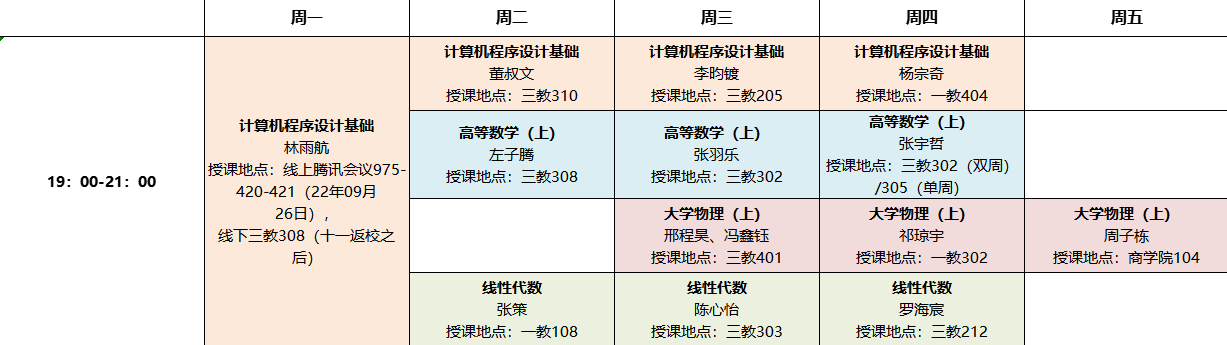
\includegraphics[width=0.75\textwidth]{arrangement.png}
\end{figure}

Come here if you want to learn more and get better grades in these courses, but to be careful with your time arrangement. Feel free to attend these classes, no scores will be graded here!

\end{frame}

\begin{frame}{QQ Group}
\begin{figure}
    \centering
    
\includegraphics[width=0.3\textwidth]{QR.jpg}
\end{figure}
\textbf{Please scan the QR code above to enter the QQ group.}

Feel free to ask questions in that QQ group. Help others and improve yourself by participating the discussions. Some review slides will be released in QQ group before the exam, hope these materials can help you!

\end{frame}

\begin{frame}{About Me...}
\begin{itemize}
    \item \textbf{Name}: Zhang Ce
    \item \textbf{Grade}: 3
    \item \textbf{Department}: Electrical and Electronic Engineering
    \item \textbf{Major}: Communication Engineering
    \item \textbf{E-Mail}: 11910803@mail.sustech.edu.cn
    \item Get $100 (A+)$ in Linear Algebra A, Fall 2019. \\
    \vspace{3pt}
    Midterm Exam: $100/100$ \qquad Final Exam: $100+/110$
    \item Contact me directly on QQ (recommended) or email if you have problems on this course or issues about major selection.
    \item I'm not your instructor, I'm just one of your schoolmates. I will try my best to prepare and give my lectures, and I can always learn from you at the same time.
\end{itemize}

\end{frame}

\begin{frame}{About This Course...}
\begin{itemize}
    \item \textbf{Course Name}: Linear Algebra A / B
    \item \textbf{Course Code}: MA107A / MA107B
    \item \textbf{Course Category}: GR (General Education Required Course)
    \item \textbf{Class Hours}: 64 \qquad \textbf{Total Credits}: 4
    \item \textbf{Assessment}: '334' Grading System \quad $60\%$ to pass this course\\
        \vspace{5pt}
        $30\%$ Regular Performance\\
        \vspace{3pt}
        \quad - $5\%$ Attendance (lectures \& tutorials since Week 4, $0.13\%$ each)\\
        \vspace{3pt}
        \quad - $15\%$ Quiz (4 times, $3.75\%$ each)\\
        \vspace{3pt}
        \quad - $10\%$ Assignments (every week, $0.7\%$ each)\\
        \vspace{3pt}
        $30\%$ Midterm Exam \\
        \vspace{3pt}
        $40\%$ Final Exam
\end{itemize}

\end{frame}
\begin{frame}{A General Overview of Linear Algebra}
\textbf{You will learn:}
\begin{itemize}
    \item \textbf{Chapter 1}: Matrices and Gaussian Elimination
    \item \textbf{Chapter 2}: Vector Spaces
    \item \textbf{Chapter 3}: Orthogonality\\
    \vspace{4pt}
-------------------------- Midterm Exam --------------------------
    \item \textbf{Chapter 4}: Determinants
    \item \textbf{Chapter 5}: Eigenvalues and Eigenvectors
    \item \textbf{Chapter 6}: Definiteness and Singular Value Decomposition
    \\
    \vspace{4pt}
--------------------------- \ Final Exam \ ---------------------------
\end{itemize}
\end{frame}

\begin{frame}{Materials Recommended}
\begin{itemize}
    \item  Gilbert Strang, MIT 18.06, Linear Algebra (Spring 2005) \\
    \url{https://www.bilibili.com/video/BV1zx411g7gq}
    \item Essence of Linear Algebra \textit{-- by 3Blue1Brown} \\
    \url{https://www.bilibili.com/video/BV1ys411472E}
\end{itemize}

\begin{figure}
    \centering
    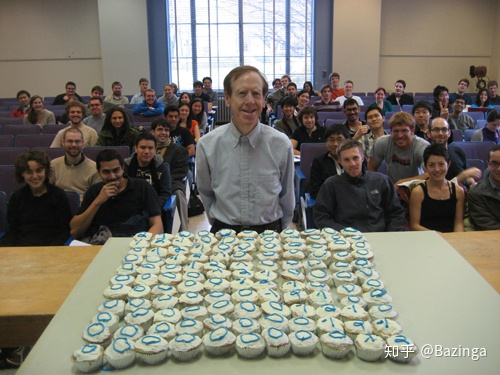
\includegraphics[width=0.6\textwidth]{Gilbert.jpeg}
\end{figure}

\end{frame}

\begin{frame}{Further Study}
\textbf{When finishing this course...}
\vspace{5pt}

Gilbert Strang, MIT, A 2020 Vision of Linear Algebra (Spring 2020)
\url{https://www.bilibili.com/video/BV1GA411t7rL}
\vspace{5pt}

For those who will major in engineering, try these courses:
\begin{itemize}
    \item EE104 Fundamentals of Electric Circuits
    \item MA201b Ordinary Differential Equations B
    \item PHY203-15 Mathematical Methods in Physics
    \item CS405 Machine Learning
\end{itemize}

For those who will major in mathematics, try these courses:
\begin{itemize}
    \item MA109 Advanced Linear Algebra
    \item MA201a Ordinary Differential Equations A
\end{itemize}


\end{frame}

\section{The Geometry of Linear Equations}
\begin{frame}{Linear Equations}


\begin{examples}
Consider this linear equations system with 2 unknowns and 2 equations,
\begin{equation*}
    \begin{cases}
	2x-y=0\\
	-x+2y=3\\
\end{cases}
\end{equation*}
Solve the values of $x$, $y$.
\end{examples}

\textbf{Equivalent Matrix Form:}

\begin{equation*}
    \left[ \begin{matrix}
	2&		-1\\
	-1&		2\\
\end{matrix} \right] \left[ \begin{array}{c}
	x\\
	y\\
\end{array} \right] =\left[ \begin{array}{c}
	0\\
	3\\
\end{array} \right]
\end{equation*}

\begin{equation*}
    A\mathbf{x}=\mathbf{b}
\end{equation*}

Try to understand it in geometric way.
\end{frame}

\begin{frame}{Row Picture}
\vspace{-5pt}
\begin{equation*}
    \begin{cases}
	2x-y=0\\
	-x+2y=3\\
\end{cases}
\end{equation*}

Every row (equation) represents a single straight line.

The problem is to find the intersection of those straight lines.

\begin{figure}
    \centering
    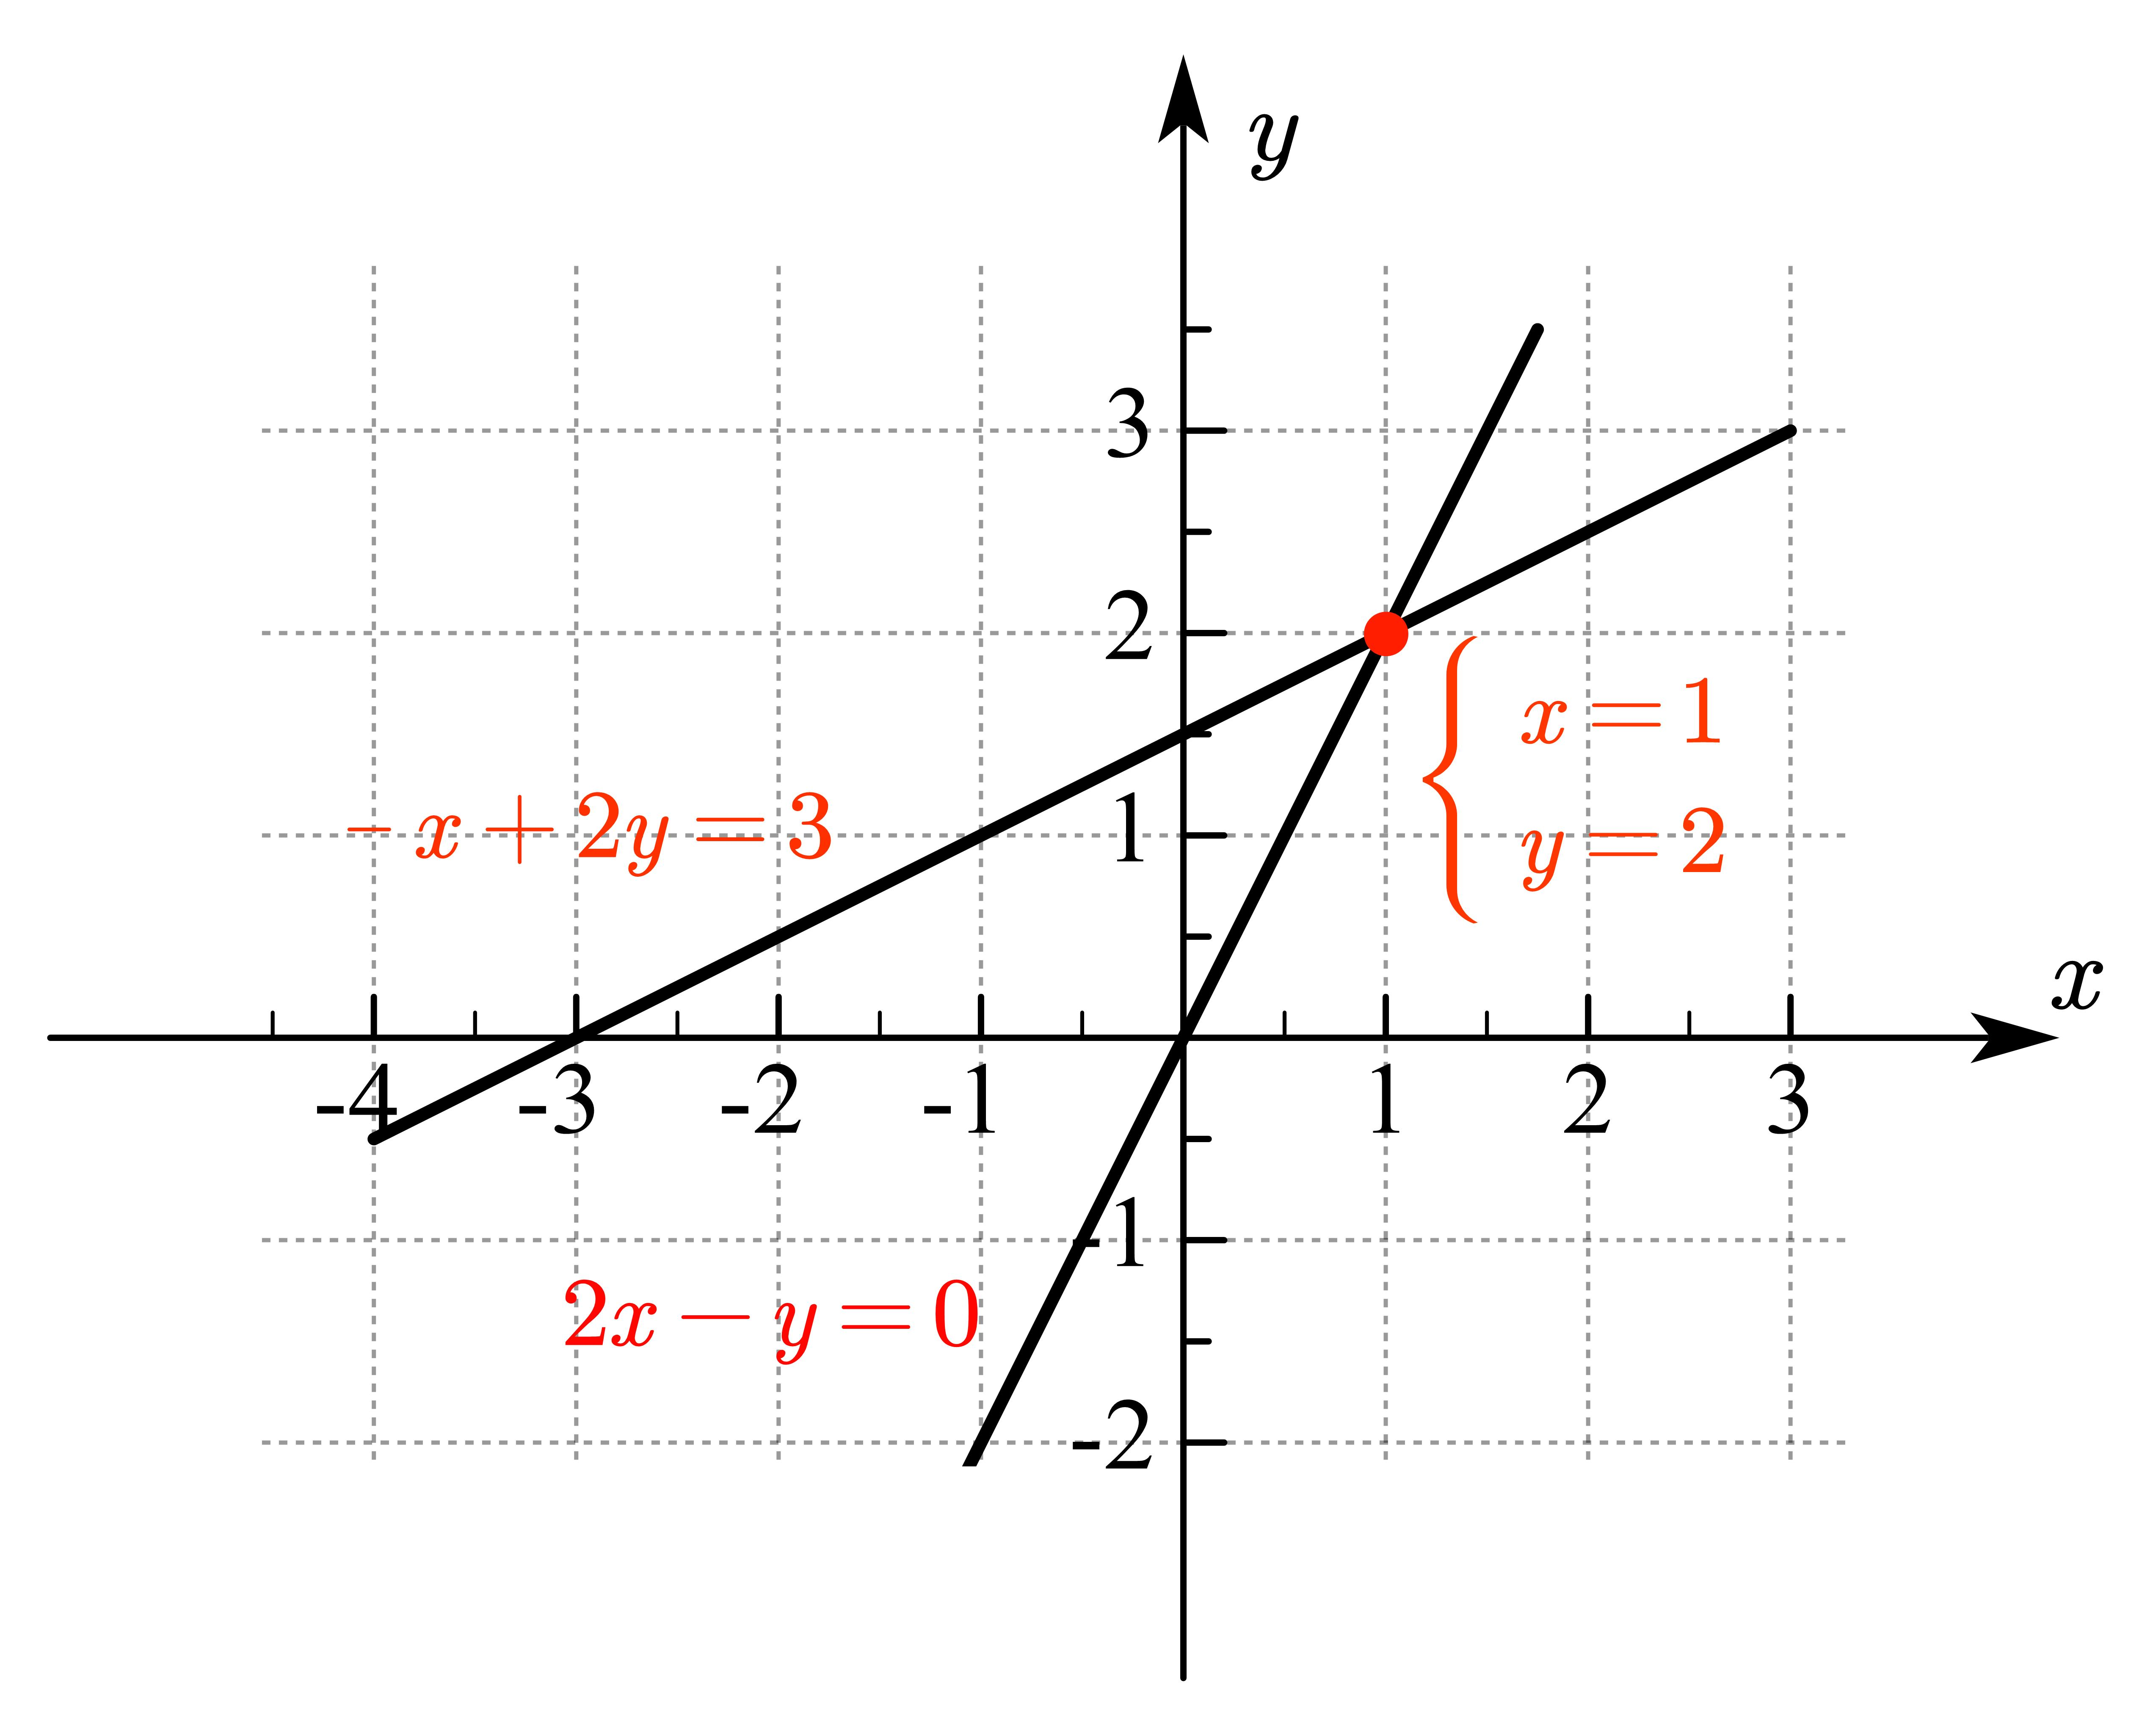
\includegraphics[width=0.55\textwidth]{Row.jpg}
\end{figure}

\end{frame}

\begin{frame}{Column Picture}
\begin{columns}
\column{0.5\textwidth}
\begin{equation*}
    \begin{cases}
	2x-y=0\\
	-x+2y=3\\
\end{cases}
\end{equation*}

\column{0.5\textwidth}
\vspace{-9pt}
\begin{equation*}
    x\left[ \begin{array}{c}
	2\\
	-1\\
\end{array} \right] +y\left[ \begin{array}{c}
	-1\\
	2\\
\end{array} \right] =\left[ \begin{array}{c}
	0\\
	3\\
\end{array} \right]
\end{equation*}
\end{columns}

\vspace{4pt}
Every column (coefficients of a single variable) represents a vector.

The problem is to find the \textbf{Linear Combination} of those vectors.
\vspace{-1.03pt}

\begin{figure}
    \centering
    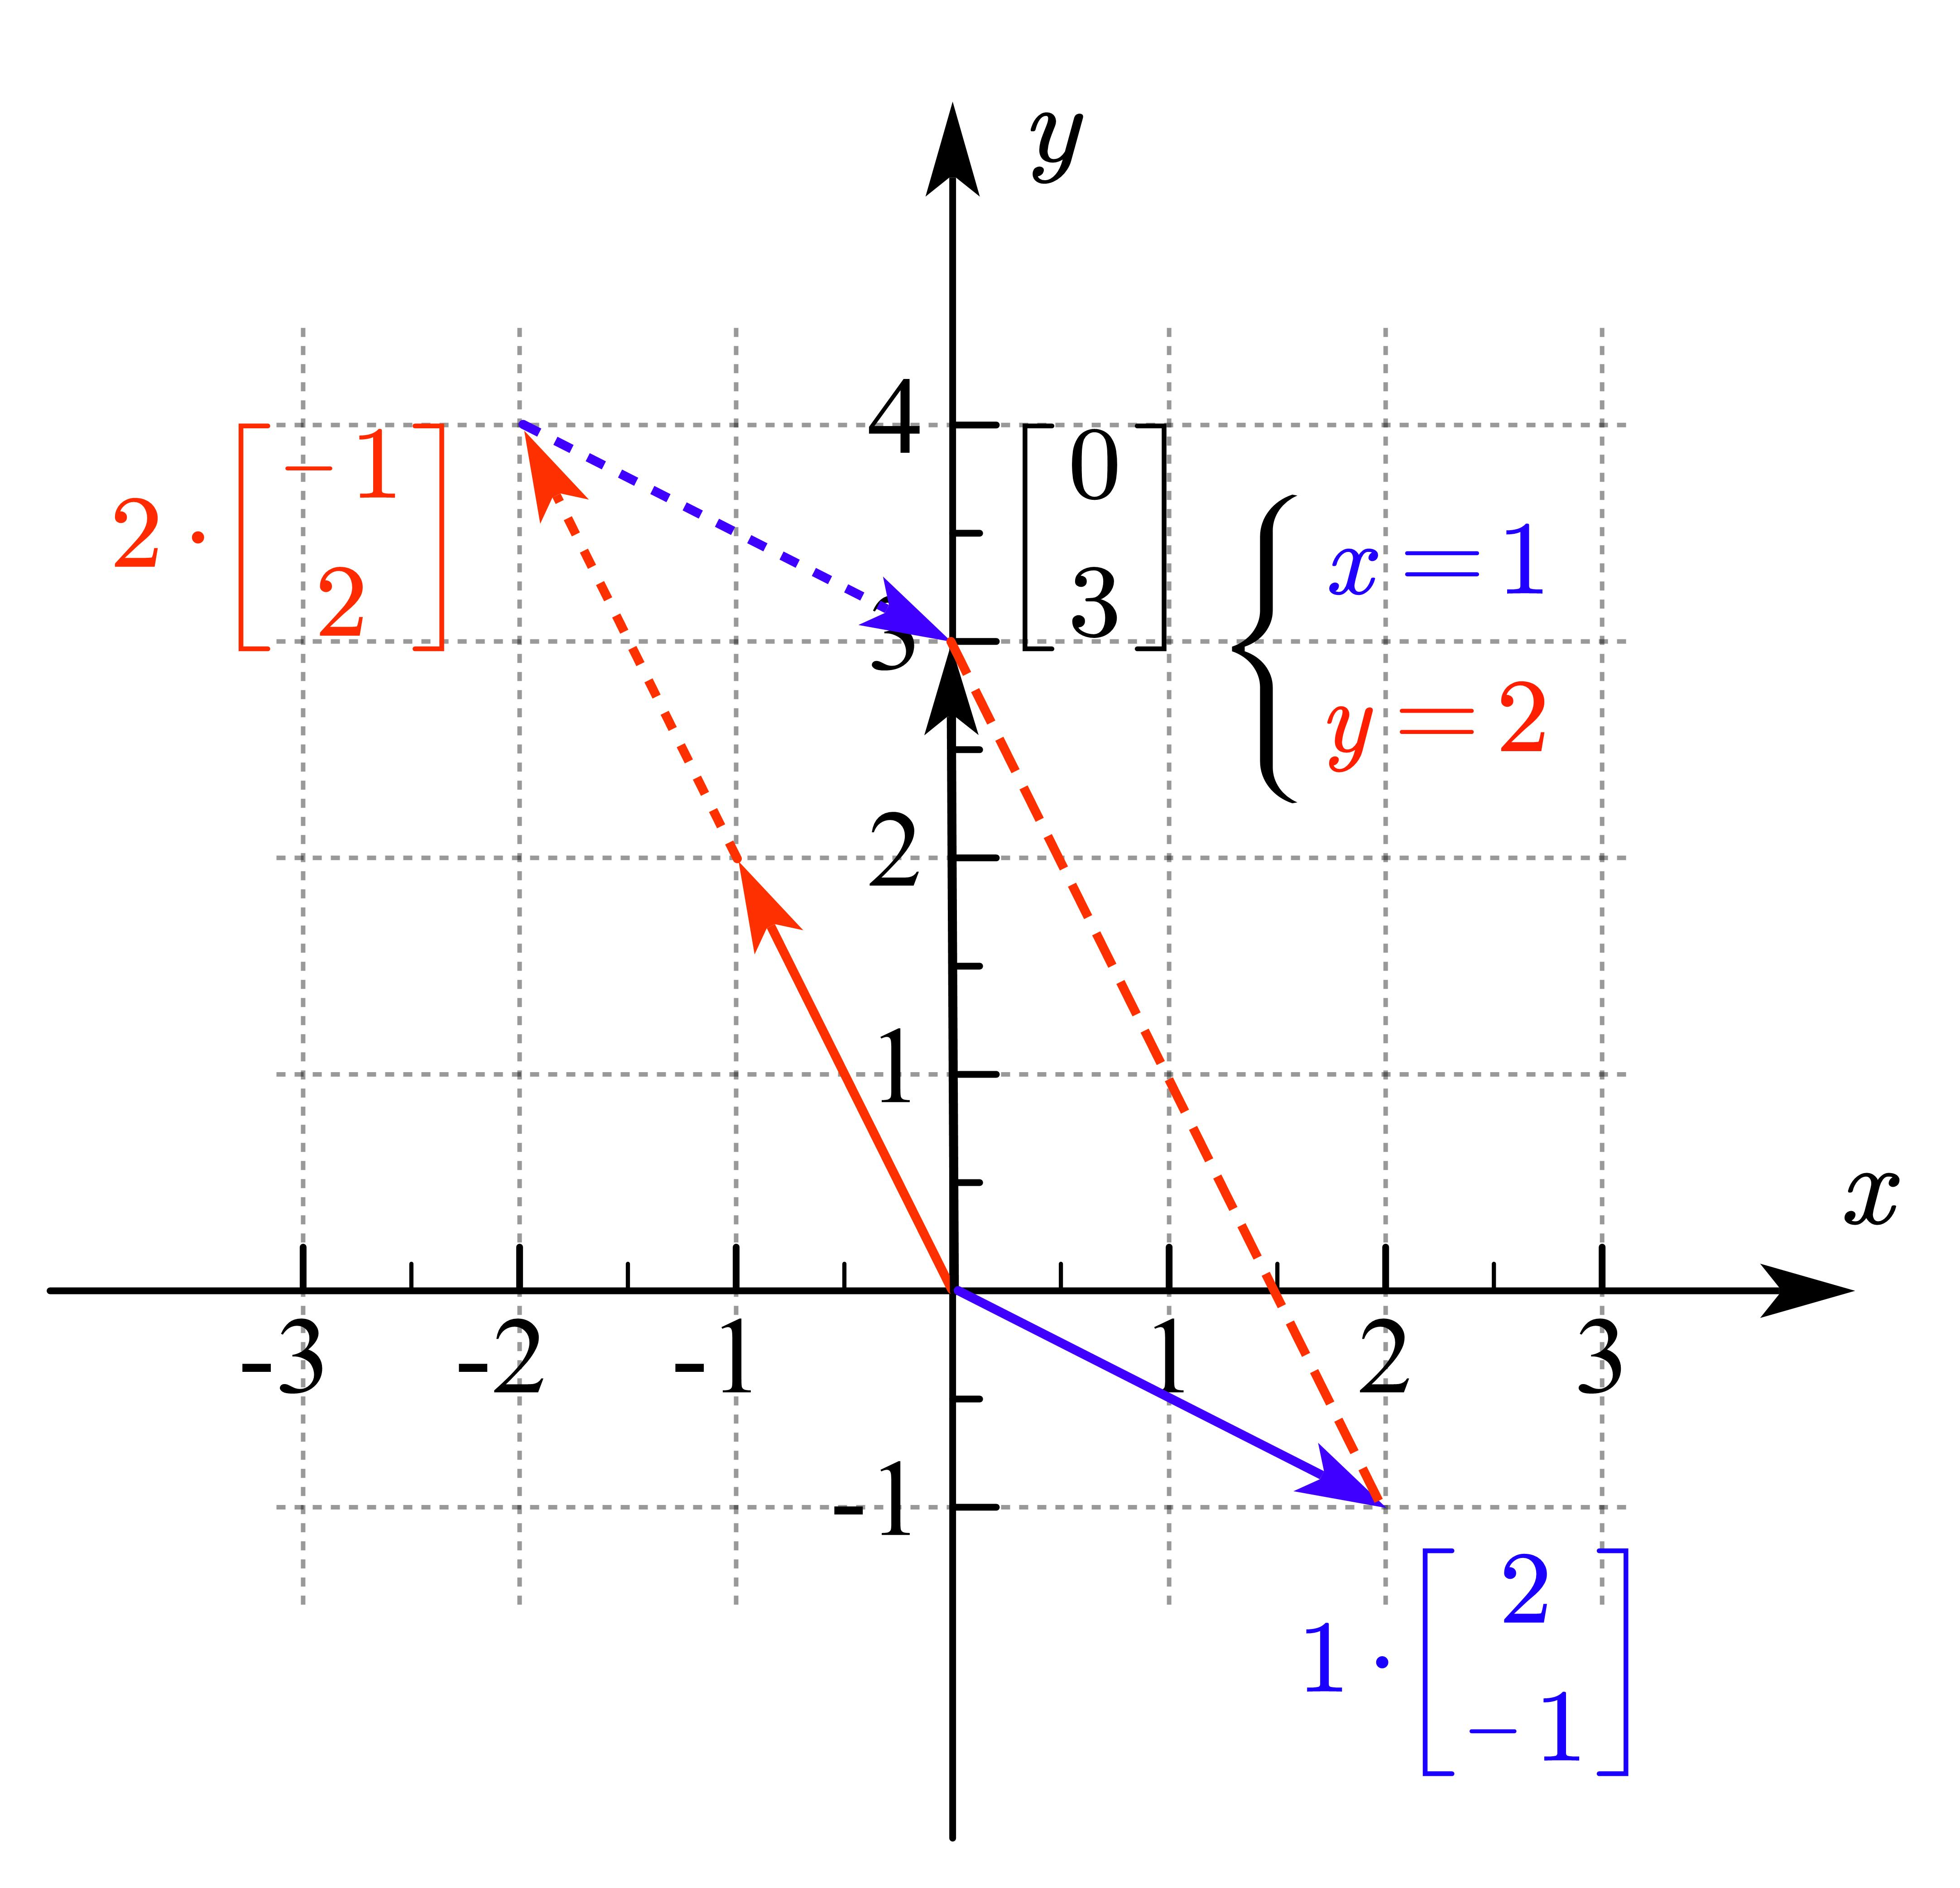
\includegraphics[width=0.48\textwidth]{Column.jpg}
\end{figure}

\end{frame}

\section{Gaussian Elimination and Back-Substitution}
\begin{frame}{Gaussian Elimination}
The core problem of linear algebra is to solve linear equations.

Consider the following system of linear equations:

\begin{equation*}
    \begin{cases}
        x+2y+z=2\\
        3x+8y+z=12\\
        4y+z=2\\
    \end{cases}
\end{equation*}

Augmented matrix:
\begin{equation*}
    \left[ \begin{matrix}
        1&		2&		1&		2\\
        3&		8&		1&		12\\
        0&		4&		1&		2\\
    \end{matrix} \right]
\end{equation*}

How can we solve it?
\end{frame}

\begin{frame}{Gaussian Elimination}
Eliminate entry on position $(2,1)$:
\begin{equation*}
    \left[ \begin{matrix}
        1&		2&		1&		2\\
        0&		2&		-2&		6\\
        0&		4&		1&		2\\
    \end{matrix} \right]
\end{equation*}

Eliminate entry on position $(3,1)$:
\begin{equation*}
    (0, skip \: this \: step)
\end{equation*}

Eliminate entry on position $(3,2)$:
\begin{equation*}
    \left[ \begin{matrix}
        1&		2&		1&		2\\
        0&		2&		-2&		6\\
        0&		0&		5&		-10\\
    \end{matrix} \right]
\end{equation*}

Elimination process done! Find the pivots above.
\end{frame}


\begin{frame}{Back-Substitution}
After elimination, we get
\begin{columns}
    \column{0.5\textwidth}
    \begin{equation*}
        \left[ \begin{matrix}
            1&		2&		1&		2\\
            0&		2&		-2&		6\\
            0&		0&		5&		-10\\
        \end{matrix} \right]
    \end{equation*}

    \column{0.5\textwidth}
    \begin{equation*}
        \begin{cases}
            x+2y+z=2\\
            2y-2z=6\\
            5z=-10\\
        \end{cases}
    \end{equation*}
\end{columns}
Do back-substitution, we can get the solution:
\begin{equation*}
    \begin{cases}
        x=2\\
        y=1\\
        z=-2\\
    \end{cases}
\end{equation*}

Rethink the whole elimination process, are there exist some cases to let the elimination process break down?
\end{frame}

\begin{frame}{Singular Cases for Gauss Elimination}
The matrix we used above is a "good" matrix.
\begin{equation*}
    \left[ \begin{matrix}
        1&		2&		1&		2\\
        3&		8&		1&		12\\
        0&		4&		1&		2\\
    \end{matrix} \right]
\end{equation*}

If we slightly change one of the element\dots
\begin{equation*}
    \left[ \begin{matrix}
        1&		2&		1&		2\\
        3&		6&		1&		12\\
        0&		4&		1&		2\\
    \end{matrix} \right]
\end{equation*}

What will happen now?
\end{frame}

\begin{frame}{Singular Cases for Gauss Elimination}
Eliminate entry on position $(2,1)$:
\begin{equation*}
    \left[ \begin{matrix}
        1&		2&		1&		2\\
        0&		0&		-2&		6\\
        0&		4&		1&		2\\
    \end{matrix} \right]
\end{equation*}

Eliminate entry on position $(3,1)$:
\begin{equation*}
    (0, skip \: this \: step)
\end{equation*}

Eliminate entry on position $(3,2)$:
\begin{equation*}
    Something \: strange \: happens.
\end{equation*}

Elimination process fails! Row exchange to fix.

\end{frame}

\begin{frame}{Singular Cases for Gauss Elimination}
Another change to make the "good" matrix singular:
\begin{equation*}
    \left[ \begin{matrix}
        1&		2&		1&		2\\
        3&		8&		1&		12\\
        0&		4&		-4&		2\\
    \end{matrix} \right]
\end{equation*}

Eliminate entry on position $(2,1)$:
\begin{equation*}
    \left[ \begin{matrix}
        1&		2&		1&		2\\
        0&		2&		-2&		6\\
        0&		4&		-4&		2\\
    \end{matrix} \right]
\end{equation*}

Eliminate entry on position $(3,2)$:
\begin{equation*}
    \left[ \begin{matrix}
        1&		2&		1&		2\\
        0&		2&		-2&		6\\
        0&		0&		0&		-10\\
    \end{matrix} \right]
\end{equation*}

Elimination process fails! Missing pivots. No method to fix.

\end{frame}

\begin{frame}{Singular Cases for Gauss Elimination}
Two kind of singular cases that can let Gauss elimination break down:
\begin{itemize}
    \item Temporal failure: Can be fixed by row exchange.
    \item Permanent failure: Missing pivots. No method to fix.
\end{itemize}

\vspace{7pt}
Recall the problem you meet in assignment:

\vspace{5pt}
Which three numbers of $k$ does elimination break down?
\begin{equation*}
    \begin{cases}
        kx+3y=6\\
        3x+ky=-6\\
    \end{cases}
\end{equation*}

$k=0$ laeds to temporal failure, while $k=3\:or\:k=-3$ leads to permanent failure.

\end{frame}

\section{Matrix Multiplication}
\begin{frame}{Matrix Size in Matrix Multiplication}
Matrix $A$: $(m \times n)$, Matrix $B$: $(n \times p)$.

\vspace{3pt}
The size of $AB$: $(m \times p)$.

\vspace{3pt}
Consider the following multiplications, are they legal?

\begin{equation*}
    \left[ \begin{array}{c}
        1\\
        2\\
        5\\
    \end{array} \right] \left[ \begin{matrix}
        1&		2&		5\\
    \end{matrix} \right] , \left[ \begin{matrix}
        1&		2&		5\\
    \end{matrix} \right] \left[ \begin{array}{c}
        1\\
        2\\
        5\\
    \end{array} \right] , \left[ \begin{matrix}
        1&		2\\
        3&		3\\
        2&		1\\
    \end{matrix} \right] \left[ \begin{array}{c}
        1\\
        2\\
        3\\
    \end{array} \right]
\end{equation*}

\begin{equation*}
    \left[ \begin{matrix}
        1&		2\\
        3&		3\\
        2&		1\\
    \end{matrix} \right] \left[ \begin{array}{c}
        3\\
        7\\
    \end{array} \right] , \left[ \begin{matrix}
        3&		3\\
        5&		4\\
    \end{matrix} \right] \left[ \begin{matrix}
        4&		5&		6&		2\\
        3&		2&		4&		3\\
    \end{matrix} \right], \left[ 5 \right] \left[ \begin{array}{c}
        3\\
        2\\
        1\\
    \end{array} \right]
\end{equation*}

The size of the multiplication result will be...

Now, I will introduce 4 methods to calculate matrix multiplication.
\end{frame}

\begin{frame}{Matrix Multiplication - 4 Methods}
Example:

\begin{equation*}
    \left[ \begin{matrix}
        3&		-1\\
        1&		4\\
    \end{matrix} \right] \left[ \begin{matrix}
        2&		1\\
        1&		2\\
    \end{matrix} \right] =\left[ \begin{matrix}
        5&		1\\
        6&		9\\
    \end{matrix} \right]
\end{equation*}

\begin{enumerate}
    \item The regular (row-col) way. (Row of A) multiply (Column of B).
    \item The row way. Linear combination of (Row of B).
    \item The column way. Linear combination of (Column of A).
    \item The col-row way. (Column of A) multiply (Row of B).
\end{enumerate}

There is also an additional method: block method.

\vspace{3pt}
When you calculate matrix multiplication in the exam, please remember to choose another method for verification.
\end{frame}

\section{LU Factorization}
\begin{frame}{Elimination Matrices}
Now it's time to understand elimination matrices. The goal is to express the elimination process by matrix language.

\vspace{3pt}
For example, to eliminate $(2,1)$ position element:
\begin{equation*}
    \left[ \begin{matrix}
        1&		2&		1\\
        3&		8&		1\\
        0&		4&		1\\
    \end{matrix} \right] \rightarrow \left[ \begin{matrix}
        1&		2&		1\\
        0&		2&		-2\\
        0&		4&		1\\
    \end{matrix} \right]
\end{equation*}

What we have done: (Row 2) - 3 (Row 1).

\vspace{3pt}
Use a elimination matrix $E_{21}$ to represent this process:

\begin{equation*}
    \left[ \begin{matrix}
        1&		0&		0\\
        -3&		1&		0\\
        0&		0&		1\\
    \end{matrix} \right] \left[ \begin{matrix}
        1&		2&		1\\
        3&		8&		1\\
        0&		4&		1\\
    \end{matrix} \right] =\left[ \begin{matrix}
        1&		2&		1\\
        0&		2&		-2\\
        0&		4&		1\\
    \end{matrix} \right]
\end{equation*}

\begin{equation*}
    E_{21}A=A'
\end{equation*}

As you might discover, $E_{32}E_{31}E_{21}A=U$.
\end{frame}

\begin{frame}{Gauss Elimination Represented in Elimination Matrices}
The process of Gauss Elimination we introduced before:
\begin{equation*}
    \left[ \begin{matrix}
        1&		2&		1\\
        3&		8&		1\\
        0&		4&		1\\
    \end{matrix} \right] \xrightarrow{r2-3r1}\left[ \begin{matrix}
        1&		2&		1\\
        0&		2&		-2\\
        0&		4&		1\\
    \end{matrix} \right] \rightarrow \left[ \begin{matrix}
        1&		2&		1\\
        0&		2&		-2\\
        0&		4&		1\\
    \end{matrix} \right] \xrightarrow{r3-2r2}\left[ \begin{matrix}
        1&		2&		1\\
        0&		2&		-2\\
        0&		0&		5\\
    \end{matrix} \right]
\end{equation*}

Gauss Elimination represented in multipling elimination matrices:
\begin{equation*}
    \left[ \begin{matrix}
        1&		0&		0\\
        0&		1&		0\\
        0&		-2&		1\\
    \end{matrix} \right] \left[ \begin{matrix}
        1&		0&		0\\
        0&		1&		0\\
        0&		0&		1\\
    \end{matrix} \right] \left[ \begin{matrix}
        1&		0&		0\\
        -3&		1&		0\\
        0&		0&		1\\
    \end{matrix} \right] \left[ \begin{matrix}
        1&		2&		1\\
        3&		8&		1\\
        0&		4&		1\\
    \end{matrix} \right] =\left[ \begin{matrix}
        1&		2&		1\\
        0&		2&		-2\\
        0&		0&		5\\
    \end{matrix} \right]
\end{equation*}

We define $E=E_{32}E_{31}E_{21}$, then we can get $EA=U$.

\vspace{3pt}
Finally we can get $A=LU$, $L=E^{-1}={E_{21}}^{-1}{E_{31}}^{-1}{E_{32}}^{-1}$.

\vspace{3pt}
Remind that $E_{21},E_{31},...,L$ are all lower triangular matrices.
\end{frame}

\begin{frame}{Why $A=LU$, not $EA=U$?}
    
\end{frame}
\end{document}